\chapter{Architecture overview}
\lhead{\emph{Appendices}} 
\label{app:arch-overview}	

The learning environment used during the experiments is inspired by the OpenAI multi-agent environment \cite{lowe_multi-agent_2017}. The simulation can be separated into distinct parts. The \textit{world} is the abstract concept where the agents will interact with each other. The second part of the architecture is involved into the reinforcement learning process. It is separated into \textit{scenarios} and \textit{runners}. Figure~\ref{fig:architecture-overview} depicts the overall architecture. The scenarios act as an interface between the world and the runners while the latter is used to manage the necessary process for the reinforcement learning. In order to simulate the interaction between entities, discrete time steps are used. For clarity, the following assumes that cubes are being transported.

\begin{figure}[h!]
\centering
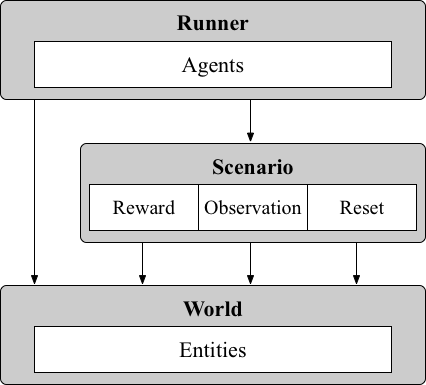
\includegraphics[width=0.5\textwidth]{imgs/architecture-overview.png}
\caption[Overview of the experiment architecture]{Overview of the experiment architecture}
\label{fig:architecture-overview}
\end{figure}

\section{World}

The world is the sandbox in which all \textit{entities} involved in an experiment will interact. Three different representations of physical objects were used. The internal state of all entities can be queried to enable the creation of the observation required by the agents. Entities can be separated into two classes. After being created, \textbf{scripted} entities will react to the changes in the environment automatically while \textbf{dynamic} entities are controlled by an external process. Dynamic entities are linked to a learning agent that will decide on the next action.   

\subsection{Buffer}
\label{sec:archi-uffer}
The buffer can be seen as a wrapper around a FIFO queue. It is the equivalent to a crate where cubes can be stocked. The size of the buffer can be limited or infinite. When there is no space left in the queue, any new element added to it will be considered lost (i.e. dropped) for the remaining of the episode.

\subsection*{Available endpoints to other entities}
\begin{enumerate}[label=(\arabic*)]
\item \textbf{get}: If a cube is available in the buffer, takes it out and returns it.
\item \textbf{put}: If space is available in the queue, puts the given cube in the buffer. Drops it otherwise.
\end{enumerate} 

\subsection*{Available state information}
\begin{itemize}[noitemsep]
\item Buffer full status (boolean)
\item Buffer empty status (boolean)
\item Current size of the queue (integer)
\item Maximum size of the queue (integer)
\end{itemize}

\subsection{Conveyor}

A conveyor acts as an automatic non-instantaneous transporter of cubes between two different points. In a nutshell, a cube placed at one end of the conveyor (\textit{head}) will be available at the other end (\textit{tail}) after a delay $t$. The head and tail of the conveyor are also buffers as described in section~\ref{sec:archi-uffer}.

The conveyor is automatic in the sense that as soon as its head buffer is full, it will start the transfer. It is assumed that the head buffer is moving along the conveyor making it unavailable for deposit during the transportation. After $t$ time steps have elapsed, the content of the head buffer will have been transferred to the tail buffer. As for a normal buffer, any cube not fitting in the tail buffer will be dropped. Similarly to the buffer entity, two endpoints are available.

\subsection*{Available endpoints to other entities}
\begin{enumerate}[label=(\arabic*)]
\item \textbf{get}: If a cube is available in the tail buffer, takes it out and returns it.
\item \textbf{put}: If space is available in the head buffer and the conveyor is not moving, puts the given cube in the buffer. Drops it otherwise.
\end{enumerate} 

\subsection*{Available state information}
\begin{itemize}[noitemsep]
\item Speed $t$ of the conveyor (integer)
\item Position of the conveyor (integer)
\item Buffer information for head buffer
\item Buffer information for tail buffer
\end{itemize}


\subsection{Robotic Arm}

The interaction with a robotic arm is done via two different controllers depicted in figure~\ref{fig:architecture-arm-controller}. The \textit{physical controller} provide a low-level API. The available endpoints in the low-level API are abstractions of the atomic actions a robotic arm can do. Such action can be moving to point $A$, gripping, releasing, etc. for example. For a more in-depth look at the physical controller, see \ref{app:ros-overview}. The low-level API is then leveraged by a \textit{meta controller} to provide high-level actions endpoints. The meta controller combines low-level actions into higher-level actions such as transporting an object from point $A$ to point $B$. In order to populate the high-level API, it is assumed that the possible pickup and deposit positions are fixed and known in advance.

\begin{figure}[H]
\centering
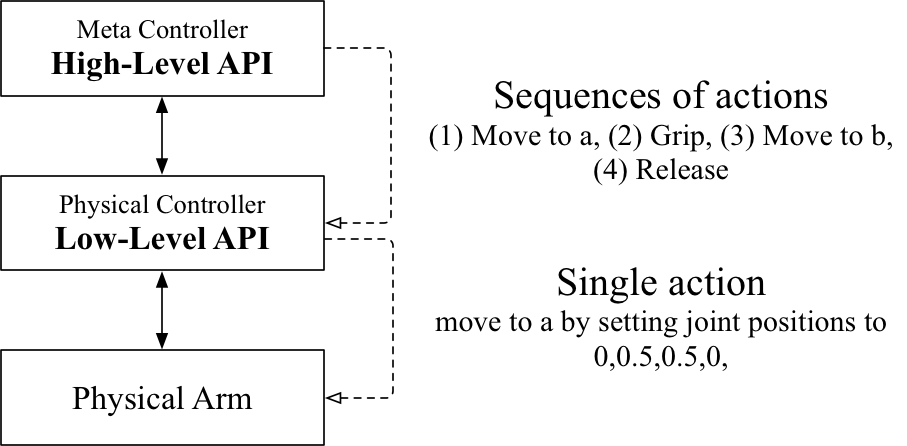
\includegraphics[width=0.7\textwidth]{imgs/ros-gazebo-archi-1.png}
\caption[Overview of the architecture used to control the robotic arms]{Overview of the architecture used to control the robotic arms}
\label{fig:architecture-arm-controller}
\end{figure}


\subsection*{Available endpoints to higher level}
\begin{enumerate}[label=(\arabic*)]
\item \textbf{$move_{p_i, d_j}$} provides endpoints to transport a cube from any pickup position $p_i$ to any deposit position $d_i$.
\item \textbf{noop} indicates to the physical controller that no action should be taken.
\end{enumerate} 

\subsection*{Available state information}
\begin{itemize}[noitemsep]
\item High-level action taken at the last time step.
\item Busy status (indicate if an low-level action is being realised)
\item Number of possible actions
\end{itemize}

\section{Scenarios \& Runners}

A scenario provides a view of the underlying world specifically tailored to the need of a reinforcement learning experiment. It creates the reward and the observation vector for each agent involved. One other duty of the scenario is to reset the world into a predefined state.

Each training session is managed by a runner. The role of the runner is to orchestrate and manage the learning. It will provide the necessary observation to the agents for their decision and update process. The runner is also in charge of indicating to the world which action should be realised in the next time step.  

\subsection{Learning Cycle}

The learning is separated into episodes. An episode can terminate either when the defined scenario is considered solved (example. no cube left to transport) or when a predefined number of steps have been done. The world is reset after each episode. The created framework is general and applies the following learning cycle.

\subsection*{Initialisation}

\begin{enumerate}[noitemsep,topsep=0pt,parsep=0pt,partopsep=0pt,label=(\arabic*)]
\item \textbf{Create the world} by creating the involved entities (buffers, conveyors, arms, etc.) as well as their relationship. Only done once per training session.
\item \textbf{Reset the world} into an initial state (ready for training). This step is repeated before each episode.
\end{enumerate}

\subsection*{Training}

The training process is managed at the runner level. The current implementation assumes that all actions and all environment changes resulting from those actions have been performed before the world moves to the next time step. 

\begin{enumerate}[noitemsep,topsep=0pt,parsep=0pt,partopsep=0pt,label=(\arabic*)]
\item \textbf{Get observation}: Get $o_t^{a_i}$ for every agent $a_i$ by querying the scenario.
\item \textbf{Action selection}: Each agent selects his action based on $o_t^{a_i}$.
\item \textbf{Apply selected action}: The selected actions are applied and all entities states are updated accordingly.
\item \textbf{Get feedback from the environment}: Based on the outcome of the actions, reward signal and next observations are constructed by the scenario.
\item If the task is considered solved (ex: no object left to transport in the system), the episode terminates. Otherwise go back to 1
\end{enumerate}

